% !TEX root = sn1604_wifes.tex

\begin{figure*}[tb!]
   \centering
   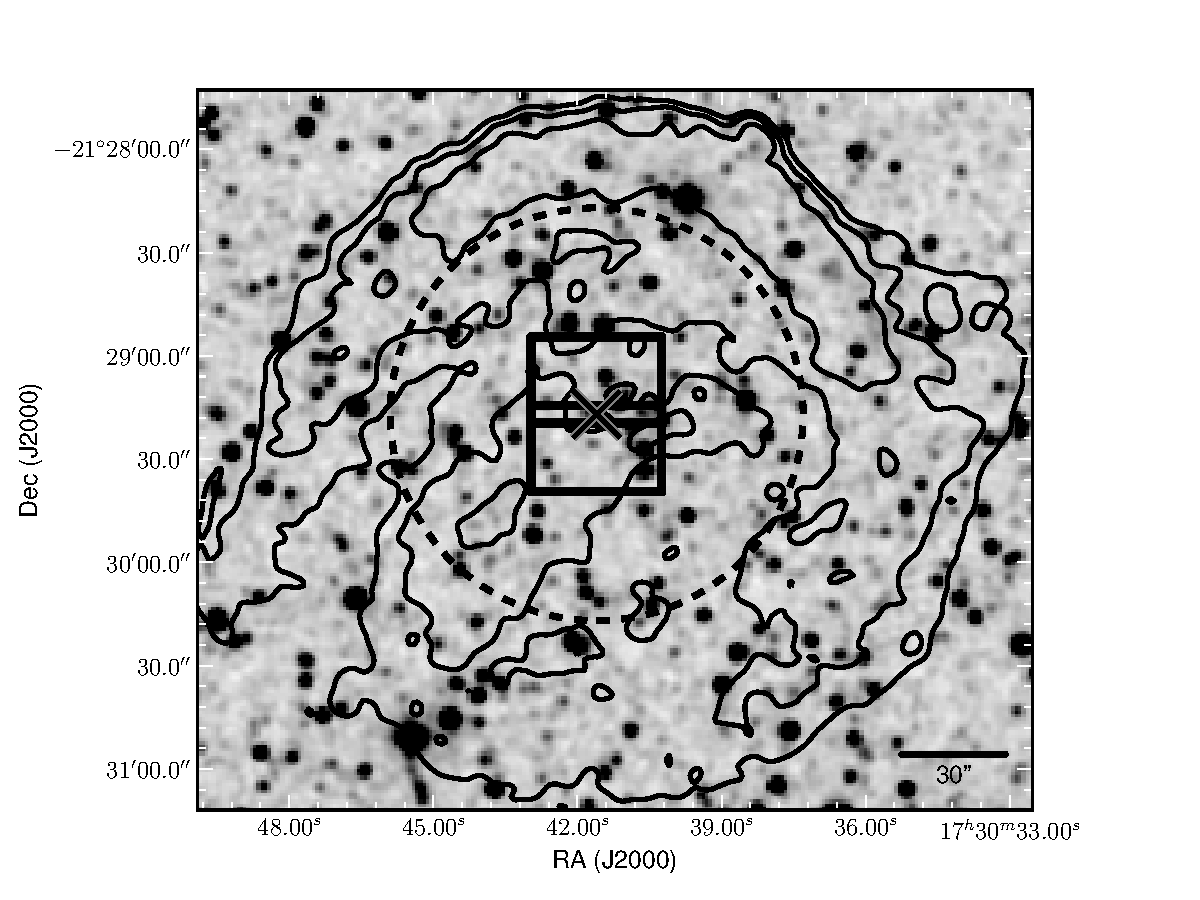
\includegraphics[width=\textwidth]{\plotdir /sn1604_overlay.pdf} 
   \caption{SN1604 \gls{2mass} image with contours of ACIS X-Ray image \citep[ObsID 116; ][]{2002ApJ...581.1101H}. In this case, 19\arcsec\ equals 1420 \kms\ at 6.4~\kpc. The dashed circle describes a 60\arcsec circle where we photometrically searched for potential companion stars.}
   \label{fig:sn1604_overlay}
\end{figure*}
